\chapter[缩放定律与效率]{缩放定律与高效大语言模型}\label{chap:scaling}

\begin{learningbox}
在本章中，你将学习语言模型的性能如何随数据与训练投入而缩放。
具体来说，你将能够：
\begin{itemize}[leftmargin=*, nosep]
    \item 解释模型性能如何通过{\em 缩放定律}与算力、数据和模型规模相关联，并预测在固定其他因素时增大某一因素的效果。
    \item 描述可用于开发{\em 更小语言模型}的技术，并分析使用更小模型在算力需求与性能上的取舍。
    \item 识别{\em 推理时算力}与训练时算力的区别。
    \item 反思\emph{可持续语言模型}以及大规模部署在环境与隐私方面的影响。
\end{itemize}
\end{learningbox}

\begin{comment}
Now that we have seen how to  design, train, and evaluate large language models, we will focus on performance: we will look beyond the models and observe general patterns related to the underlying resources required for creating them. We separate our discussion into four parts. First, we discuss how a model's performance can be predicted according to \emph{scaling laws} (Section~\ref{sec:scaling-laws}). Next, we turn to \emph{small language models} and the techniques that make them capable under resource budgets (Section~\ref{sec:small-models}). We then discuss \emph{inference-time compute}, where additional computation is spent at inference time rather than during training (Section~\ref{sec:inference-time}). Finally, we reflect on \emph{sustainable language models} and the environmental and privacy implications of large-scale deployment (Section~\ref{sec:sustainable}).
\end{comment}

\section{缩放定律：算力、数据、参数}
\label{sec:scaling-laws}
LLM 训练涉及三个主要因素：\begin{enumerate*}[label=(\arabic*)]
    \item 算力总量，
    \item 数据集规模，以及
    \item 模型规模。
\end{enumerate*}
研究表明，这三个因素与模型的最终性能（以它在留出测试集上的损失 $L$ 衡量）相关。人们发现这种关系既平滑又可预测。该关系呈\emph{幂律}形式：三者中任一资源增加时，损失按该资源的负幂次成比例下降。例如，把模型规模翻倍，可能使损失降低为原来的 $2^{-\alpha}$ 倍，其中 $\alpha$ 是某个正指数。由于这种行为是可预测的，我们可以在投入一次昂贵训练{\em 之前}，估计模型会有多大提升（例如把训练集规模翻倍带来的提升）。

我们把这三个量（$C$、$D$、$N$）定义如下：
\begin{itemize}
    \item 算力（$C$）：整个训练过程中执行的算术运算总量，以浮点运算次数（FLOPs）计。注意这是运算的总次数，而不是每秒速率。一个被广泛使用的近似关系把它与另外两个量联系起来：$C \approx 6ND$，因为处理单个词元会在前向（两次）与反向传播（四次）中大致六次触及 $N$ 个参数中的每一个。
    \item 数据集规模（$D$）：模型训练所用的词元总数。注意词元是由分词器定义的子词单位，因此同一语料在不同分词器下对应不同的 $D$。$D$ 的计数是训练过程中实际使用的词元数。当数据在若干轮次中重复时，重复的词元仍计入 $D$，但与新鲜数据相比可能收益递减。
    \item 模型规模（$N$）：模型架构中可训练参数（权重）的数量。这一计数通常只包含随模型深度缩放而增加的参数，因此不含嵌入矩阵。
\end{itemize}
训练大型模型代价不菲，通常在数千万美元的量级，算力时间可长达数月。缩放定律让我们能够预测一个模型是否能训练得好。

\begin{figure}[t]
    \centering
    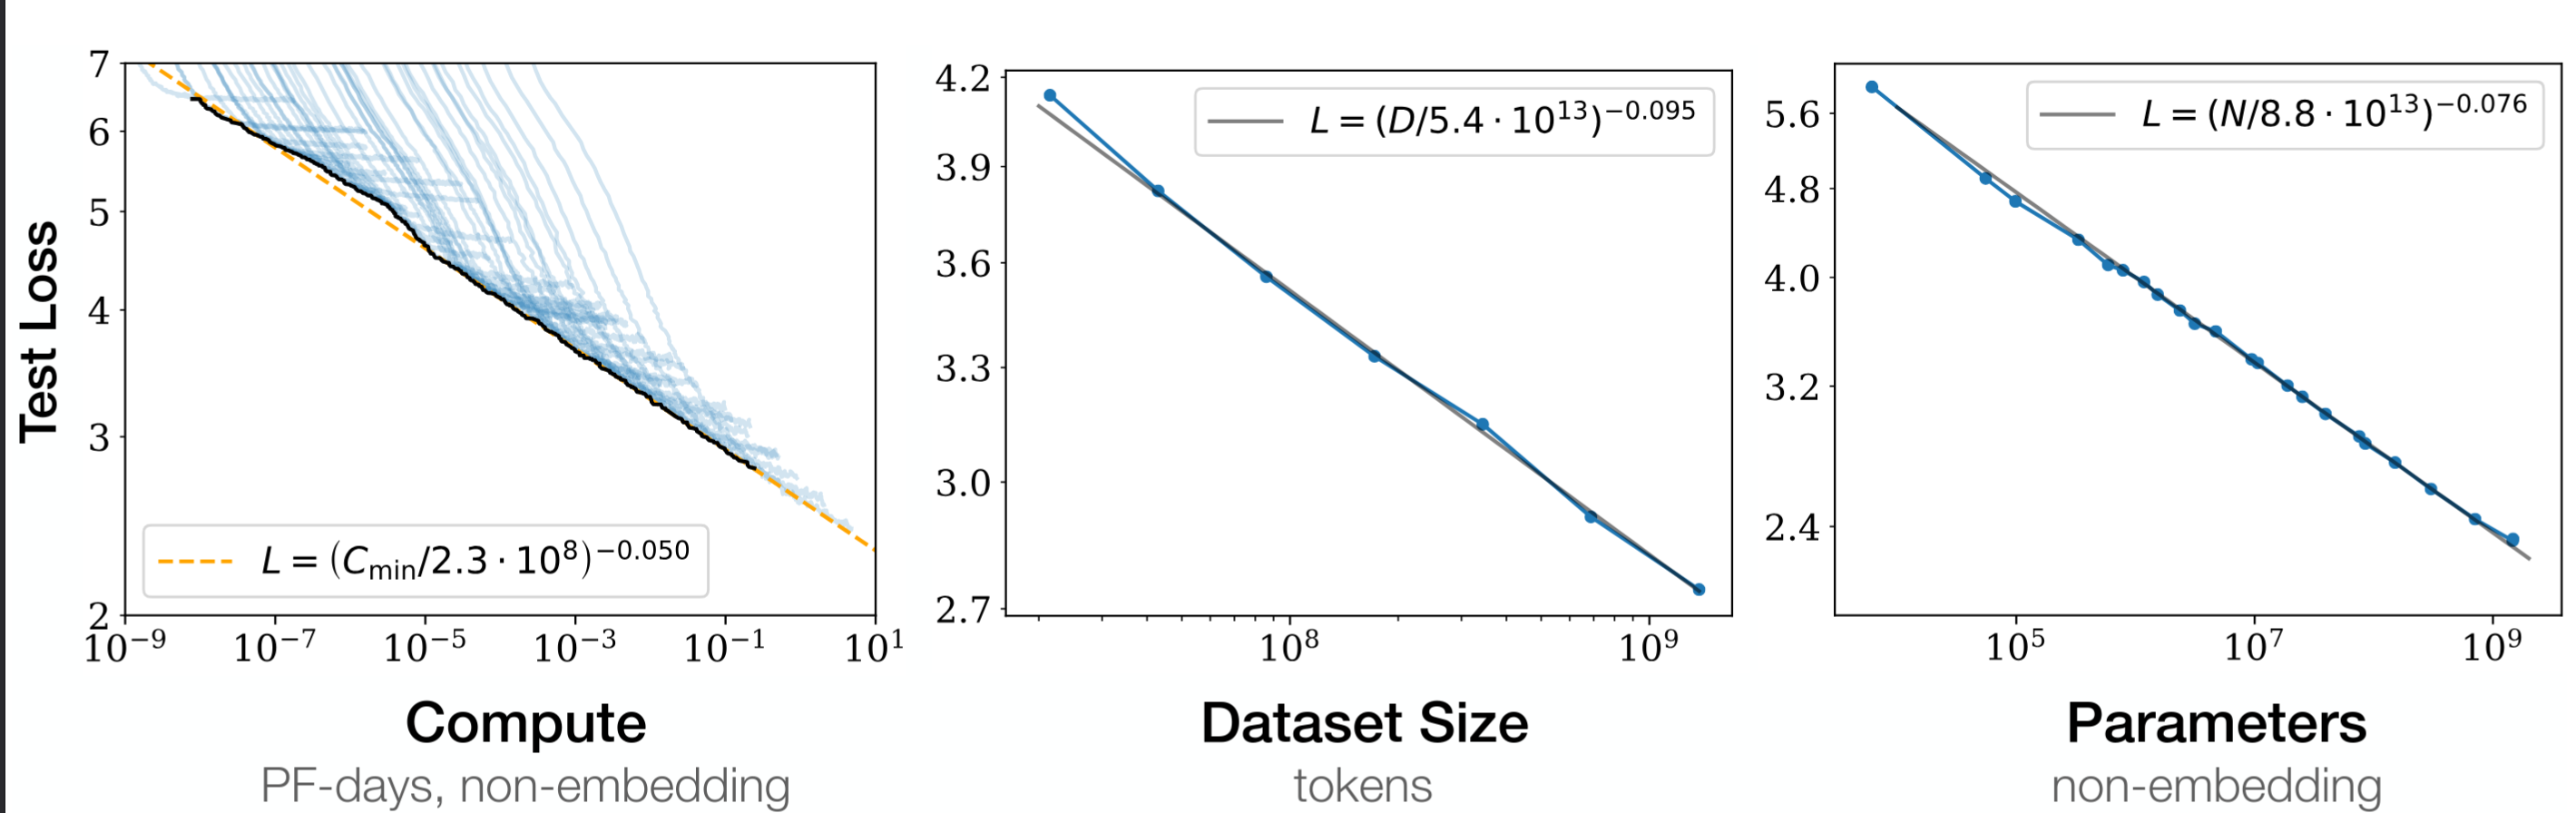
\includegraphics[width=0.9\linewidth]{part1/visuals/scaling.png}
    \caption{语言建模目标的损失是训练算力、数据集规模与模型规模的函数 \citep{kaplan2020scalinglawsneurallanguage}。}
    \label{fig:scaling-law}
\end{figure}


\subsection{Kaplan 缩放定律}
缩放定律有不同的实证结果，它们都是通过把某个函数拟合到实验测试数据上得到的。例如在图~\ref{fig:scaling-law} 中，每个点都是在一个固定数据集、相似实验设置下训练出的模型，只改变三个主要变量 $C,D,N$。2020 年初，\citet{kaplan2020scalinglawsneurallanguage} 发现了模型性能与 $C,D,N$ 的关系。
依据实证观察，他们估计损失分别与三个主要变量呈独立的幂律关系：$L(N) \propto N^{-\alpha_N}$ 与 $L(D) \propto D^{-\alpha_D}$，其中 $\alpha_N \approx 0.076$、$\alpha_D \approx 0.095$。

这些独立的幂律可以合并为一个可优化的单一方程，如式~\ref{eq:joint-power} 所示。这一关系被假定为通用的：它也能很好地充当「其他生成式建模任务」的损失行为模型 \citep[p. 5]{kaplan2020scalinglawsneurallanguage}。作者进一步表明，在除算力预算之外别无其他约束的条件下，他们的推导会给出最优模型规模 $N$ 与理想数据集规模 $D$，并由最优步长（$S$）与批大小（$B$）界定。

\begin{equation}
\label{eq:joint-power}
L(N, D) = \Big[ \Big(\frac{N_c}{N}\Big)^{\frac{\alpha_N}{\alpha_D}} + \frac{D_c}{D} \Big]^{\alpha_D}
\end{equation}

具体而言，他们得出结论：随着算力预算 $C$ 增加，模型规模 $N$ 应比数据规模 $D$ 增长得更快（$N \propto C^{0.73}$、$D \propto C^{0.27}$\footnote{$B\propto C^{0.24},\,S\propto C^{0.03},\, D=B\cdot S \propto C^{0.27}$}），这促成了 GPT-3 等大型模型的诞生。负指数反映的是收益递减：模型规模或数据集规模每翻一倍，损失只下降几个百分点。

乍看之下，这一建议似乎与指数本身相矛盾：既然 $\alpha_D > \alpha_N$，那么在算力相对增幅相同时，扩展数据比扩展参数能\emph{更快}地降低损失。原因在于约束是算力，而不是资源本身：由于 $C \approx 6ND$，增加 $D$ 与增加 $N$ 一样消耗算力。这意味着 $N$ 越来越可能成为瓶颈。因此，一旦把 $D$ 的算力代价计入，把额外算力分配给 $N$ 的回报就优于分配给 $D$。也就是说，最优分配偏向更大的模型。




\paragraph{样本效率} 
\citet{kaplan2020scalinglawsneurallanguage} 的另一个观察是：更大的模型\emph{样本效率}更高。在固定训练词元数下，更大的模型能达到更低的损失；而要达到某个目标损失，它比更小的模型所需词元更少、优化步数也更少。这一效应见图~\ref{fig:sample-efficiency-tokens}。

\begin{figure}[t]
    \centering
    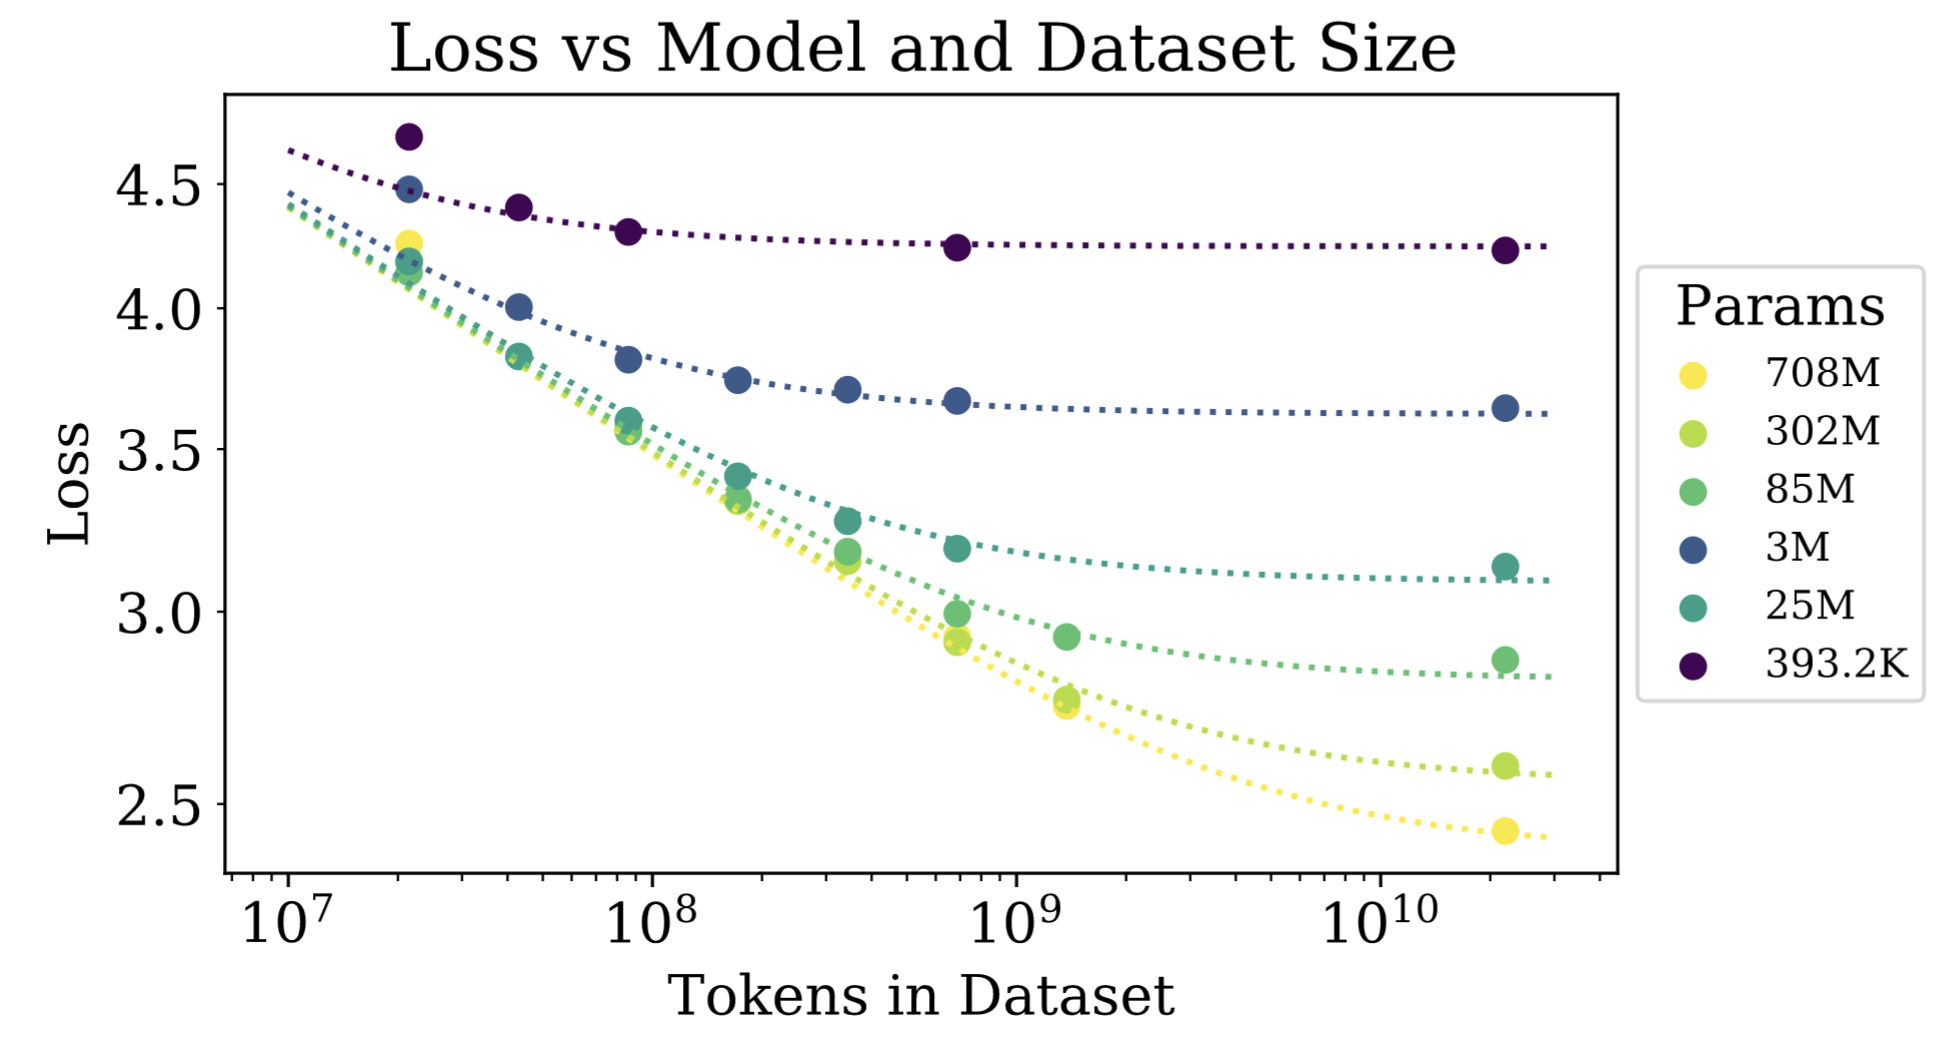
\includegraphics[width=0.7\linewidth]{part1/visuals/sample_efficiency_tokens.png}
    \caption{更大的模型用更少的训练词元即可达到给定损失，体现出更高的样本效率 \citep{kaplan2020scalinglawsneurallanguage}}
    \label{fig:sample-efficiency-tokens}
\end{figure}


\subsection{Chinchilla 缩放定律}
2022 年，\citet{10.5555/3600270.3602446} 用一个名为 Chinchilla 的模型重新评估了这些发现，并出人意料地发现：当时大多数大模型都严重训练不足。这一偏差可以追溯到 \citet{kaplan2020scalinglawsneurallanguage} 的方法论：他们的最优分配是从许多模型\emph{早期}、尚未收敛的训练动态中外推而来的，而不是从训练到收敛的运行中得出的，这系统性地把结论偏向了「用更少步数训练的更大模型」。

Chinchilla 研究的关键洞见是：算力预算每翻一倍，模型规模 $N$ 与训练词元数 $D$ 都应大致等比例增加（$N \propto C^{0.5}$、$D \propto C^{0.5}$）。他们的经验法则是：为达到算力最优，模型中每个可训练参数大约应配 20 个训练词元。这一结果此后被复现 \citep{besiroglu2024chinchilla}，并被证明对相当大的扰动依然稳健 \citep{schaeffer2025evaluating}。

在他们的缩放定律中，损失被建模为参数数量 $N$ 与已训练词元数 $D$ 的函数，如下：
\begin{equation}
    L(N,D) = E + \frac{A}{N^{\alpha}} + \frac{B}{D^{\beta}}
\end{equation}

第一项 $E$ 是不可约损失，对应自然文本的熵。第二项 $\frac{A}{N^{\alpha}}$ 刻画有限参数 $N$ 带来的次优性，最后一项 $\frac{B}{D^{\beta}}$ 刻画在有限词元数 $D$ 上训练带来的次优性。虽然这里的 $\alpha$ 与 $\beta$ 与 Kaplan 的 $\alpha_N$、$\alpha_D$ 起相同作用（即决定损失如何随模型规模与数据下降的指数），但它们是另一套参数化：它们在这两项形式中被联合拟合，因此取值不同。在 400 多个模型上拟合 Chinchilla 缩放函数，得到如下参数估计：
\begin{equation}
    E \approx 1.69, \quad A \approx 406.4, \quad B \approx 410.7, \quad \alpha \approx 0.34, \quad \beta \approx 0.28
\end{equation}

在固定算力预算 $C$ 的约束下（回想 $C \approx 6ND$）优化这一损失函数，我们可以导出任意预算 $C$ 下的算力最优模型规模 $N_{opt}$ 与数据规模 $D_{opt}$：
\begin{equation}
    N_{opt}(C) = G \left( \frac{C}{6} \right)^a, \quad D_{opt}(C) = \frac{1}{G} \left( \frac{C}{6} \right)^b
\end{equation}
其中 $G=\big(\frac{\alpha A}{\beta B}\big)^{\frac{1}{\alpha + \beta}}$ 是常数，$a = \frac{\beta}{\alpha + \beta} \approx 0.45$、$b = \frac{\alpha}{\alpha + \beta} \approx 0.55$。

注意 $a$ 与 $b$ 并不独立：按构造有 $a+b=1$。这直接来自 $C \approx 6ND$——取对数得 $\log C = \log 6 + \log N + \log D$。写成 $N_{opt} \propto C^a$、$D_{opt} \propto C^b$，则变为 $\log C = \text{const} + a \log C + b \log C$，而这对所有 $C$ 都成立的前提正是 $a+b=1$。同样的约束也适用于 Kaplan 的指数（$0.73 + 0.27 = 1$）。Chinchilla 的不同之处在于\emph{如何}在 $N$ 与 $D$ 之间分配预算。

% \paragraph{How constant is the ``20''?} The ratio is only \emph{approximately} fixed: since $D_{opt}/N_{opt} \propto C^{\,b-a}$ with $b-a \approx 0.1$, each tenfold increase in the compute budget multiplies the optimal token-to-parameter ratio by only $10^{0.1} \approx 1.26$, a change of about $26\%$ per order of magnitude. Over the practically relevant range this leaves the ratio in the ``tens of tokens per parameter'' band, which \citet{10.5555/3600270.3602446} rounded to the memorable constant $20$. 

这条法则大致是\emph{线性}的，因为 $N_{opt}$ 与 $D_{opt}$ 随算力预算 $C$ 以几乎相同的速率增长：它们的指数 $a \approx 0.45$ 与 $b \approx 0.55$ 很接近，因此比值 $D_{opt}/N_{opt}$ 在跨越许多数量级的算力范围内都保持在接近常数、约为 $20$ 的水平。
这个数值最好理解为以真实算力最优训练为锚点的经验标定，而不是一个能从拟合系数干净地推出来的数。Chinchilla 模型本身（700 亿参数、在 1.4 万亿词元上训练）恰好落在 $D/N = 20$ 上。表~\ref{tab:token-param} 给出了几个知名模型相对这条法则的位置。低于该比值的模型属于\emph{训练不足}（相对其词元预算而言过大），而远高于该比值的模型则是被刻意\emph{过度训练}，目的是得到一个小模型、在推理时运行成本低廉。更早的旗舰模型如 GPT-3 与 Gopher 远低于这条线（$D/N \approx 1$–$2$）：它们做得非常大，但相对而言训练词元太少。
% In the models Chinchilla used, to spend a compute budget optimally one should train on about $20$ tokens for every parameter; a compute-optimal $10$B-parameter model, for example, calls for on the order of $200$B training tokens.
% This was the central correction over the earlier recommendation of \citet{kaplan2020scalinglawsneurallanguage}, under which models were made very large but trained on comparatively too few tokens. 
值得强调的是，$D \approx 20N$ 仅在固定训练预算下最小化\emph{训练}损失时才最优。当模型之后要服务大量推理请求时，人们常常刻意用远超每参数 $20$ 个词元的量对它进行\emph{过度训练}，以额外的训练成本换取一个推理时运行更便宜的小模型。例如 LLaMA-3 8B 大约按每参数 $1900$ 个词元训练。这种刻意的极端过度训练，是为了让小模型仍能达到低损失，同时在推理时运行便宜。

\begin{table}
    \centering
    \begin{tabular}{lrrrl}
        \toprule
        模型 & $N$ & $D$ & $D/N$ & 状态 \\
        \midrule
        Gopher \citep{rae2021scaling}            & 280B & 300B & $\approx 1$    & 训练不足 \\
        GPT-3 \citep{brown2020language}          & 175B & 300B & $\approx 1.7$  & 训练不足 \\
        Chinchilla \citep{10.5555/3600270.3602446} & 70B  & 1.4T & $20$           & 算力最优 \\
        LLaMA-1 7B \citep{touvron2023llama1}     & 7B   & 1.0T & $\approx 143$  & 过度训练 \\
        LLaMA-2 7B \citep{touvron2023llama}      & 7B   & 2.0T & $\approx 286$  & 过度训练 \\
        LLaMA-3 8B \citep{grattafiori2024llama3herdmodels} & 8B   & 15T  & $\approx 1875$ & 过度训练 \\
        \bottomrule
    \end{tabular}
    \caption{若干知名模型相对于 Chinchilla 经验法则 $D \approx 20N$ 的词元—参数比。}
    \label{tab:token-param}
\end{table}


% Proceed with rest of section by introducing the four phenomena related to model scaling.
到目前为止，图景相当清晰：测试损失随算力、数据与参数平滑、单调且可预测地下降。然而在实践中，各种因素会影响我们的结果。我们讨论四种现象，它们各自探查这幅图景的不同边缘：
\begin{enumerate*}[label=(\arabic*)]
    \item 算力最优曲线，
    \item 涌现能力，
    \item 逆缩放，以及
    \item 顿悟（grokking）。
\end{enumerate*}
    

\subsection{算力最优曲线}
计算机硬件与能源都是有限资源。一个实际问题是如何在模型规模 $N$ 与数据集规模 $D$ 之间分配固定算力预算 $C$，以获得尽可能好的模型。缩放定律通过\emph{算力最优前沿}来回答：即最小化损失的 $C$ 的分配方式。

这一前沿通过 \emph{IsoFLOP} 方法 \citep{10.5555/3600270.3602446} 经验地确定，如图~\ref{fig:isoflop} 所示。对不同的模型规模，我们选择训练词元数，使最终 FLOPs 为常数。学习率用余弦退火调度来调整，余弦周期长度设定为与目标 FLOP 数匹配。我们在损失中发现一个明显的谷底，意味着对给定 FLOP 预算存在一个最优的待训练模型规模（左图）。利用这些谷底的位置，我们外推出更大模型的最优模型规模与词元数（中图与右图）。绿色部分给出了按 Gopher 的算力预算训练的最优模型的估计参数数与词元数。对固定 FLOP 预算，我们训练若干不同规模的模型：太小的模型欠拟合，而太大的模型被迫在过少词元上训练，于是损失随模型规模变化的曲线呈 U 形。其最小值即确定算力最优模型规模 $N_{opt}$，再由 $C \approx 6ND$ 得到匹配的词元数 $D_{opt} = C / 6N_{opt}$。对每条这样的曲线拟合抛物线即可定位该最小值，在各个预算上重复这一过程，就能发现 $N_{opt}$ 与 $D_{opt}$ 如何随算力增长。

这种抛物线拟合必须谨慎进行，该简化会在估计的最优点中引入系统性偏差 \citep{czech2026problemschinchillaapproach2}。这些偏差即便在无噪声的合成数据上也依然存在，其来源有三：（1）采样的模型规模间距过粗；（2）采样未能对称地定位真正的最小值；（3）损失曲面本身的不对称性——对称的抛物线无法表示它。在 Llama-3 的规模上，他们估计这类偏差会浪费约 140 万美元的算力。作为补救，他们建议直接拟合参数化损失模型 $L(N,D) = E + A/N^{\alpha} + B/D^{\beta}$——即 Chinchilla 方法 3，也正是我们上面用来导出 $D \approx 20N$ 法则的那种形式——并配合数值上稳健的优化器，而不是从拟合出的抛物线上读取最优点。

关于缩放的补充观点 \citep{paquette2024} 研究的是可解析求解的模型（用单遍随机梯度下降训练的幂律随机特征），而不是对已训练模型拟合曲线。他们发现，算力最优指数并非单一的普适常数，而是：数据复杂度/目标复杂度平面会分裂为四个主要相（外加三个子相），每个相都有自己的指数，决定 $N_{\mbox{opt}}$ 如何随算力增长。该采用哪条分配法则、以及固定的{\em 每参数 20 个词元}是否连形状都对，取决于问题所处的相。


\begin{figure}
    \centering
    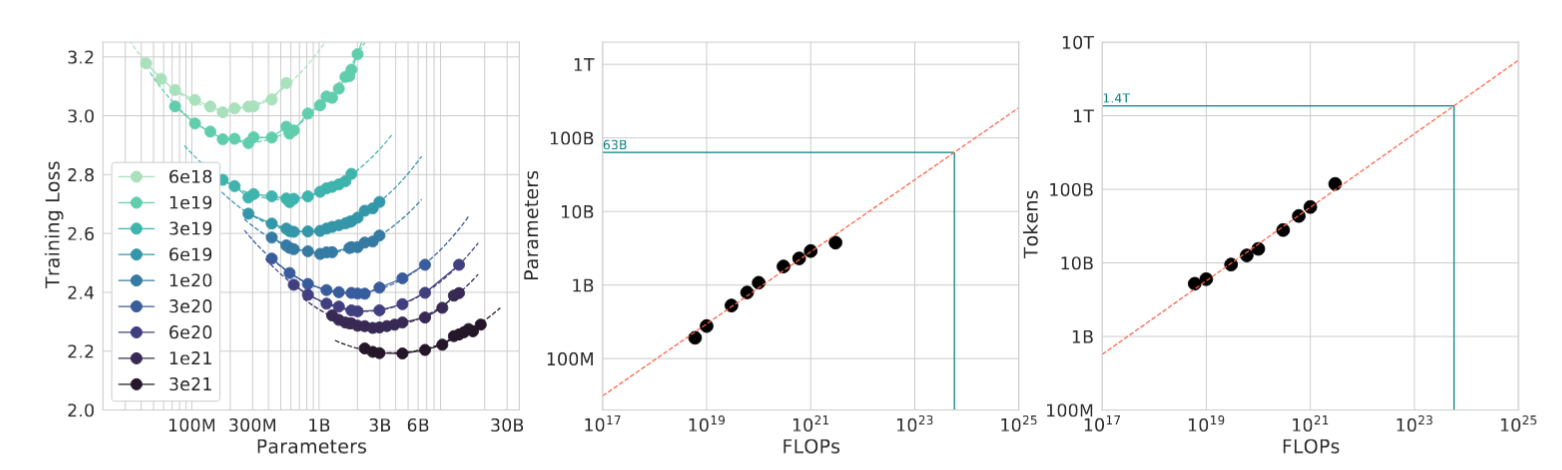
\includegraphics[width=\linewidth]{part1/visuals/isoflop.png}
    \caption{IsoFLOP 曲线  \citep{10.5555/3600270.3602446}}
    \label{fig:isoflop}
\end{figure}


\paragraph{微调的缩放}
上述工作研究的是预训练如何缩放。这些缩放定律是否也支配微调？\citet{zhang2024when} 针对全模型微调（更新模型全部权重）与参数高效微调（PEFT，冻结预训练权重、只训练一小部分新增参数，如 LoRA 所做）研究了这一问题 \citep{hu2021lora}。与算力预算最相关的一条经验是：微调性能的提升，更多来自扩展\emph{基础模型}的规模，而不是收集更多微调数据；而增加可训练的 PEFT 参数收效甚微。在实践中，一个表现不佳的任务，通常更应改为从一个更大的预训练模型出发，而不是去扩大适配器或收集更多微调样本。


\subsection{涌现能力}
LLM 缩放中最有趣的一些现象是\emph{涌现能力}：在较小模型中不存在、但当模型规模或算力越过某一阈值时突然出现的能力 \citep{wei2022emergent}。例子包括多步推理、少样本翻译以及专门的编程任务，如图~\ref{fig:emergent-abilities} 所示。当语言模型在某一规模之前只能达到随机水平、之后性能显著提升到远高于随机时，通过少样本提示完成某项任务的能力就是涌现的。

\begin{figure}
    \centering
    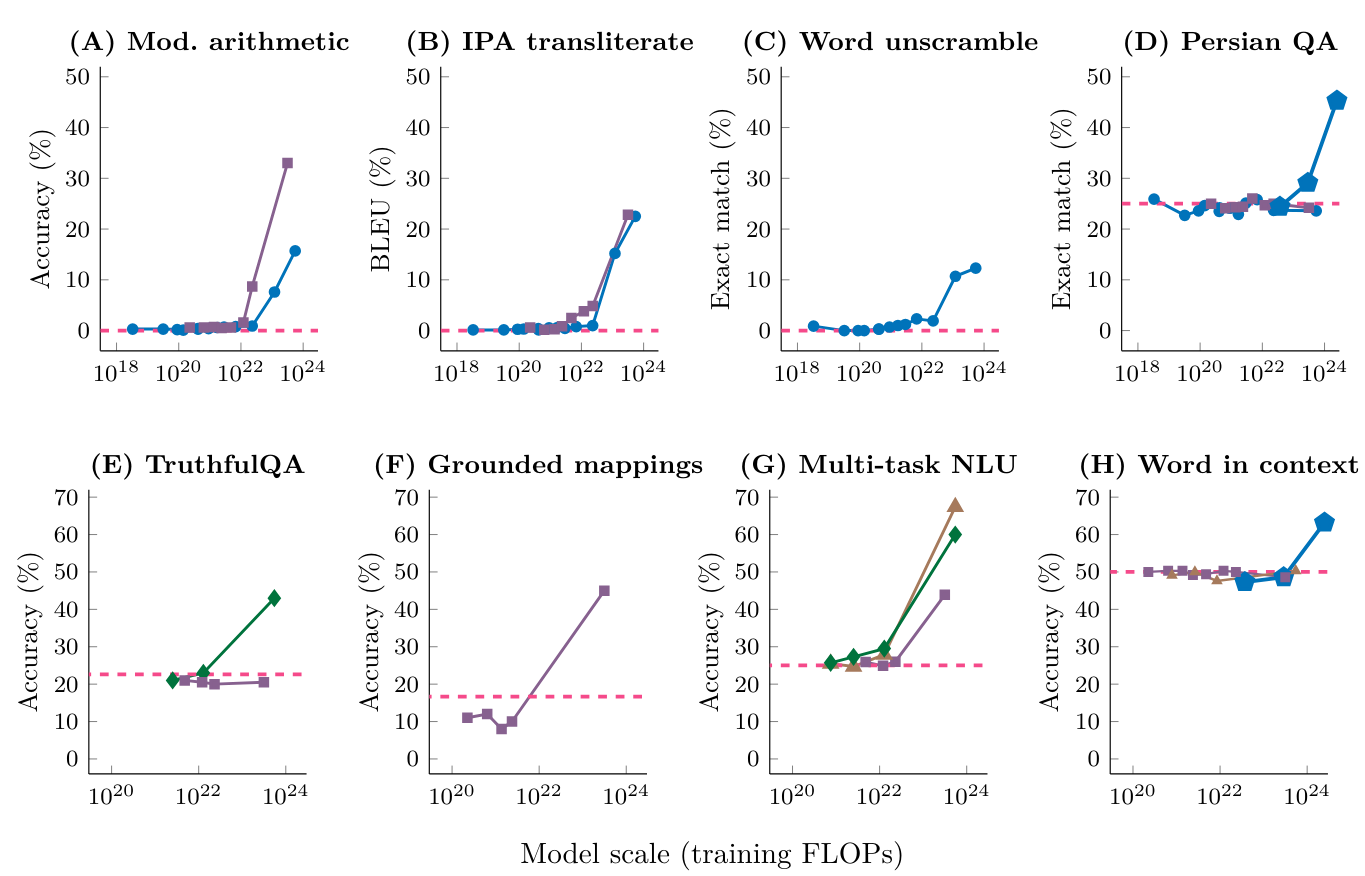
\includegraphics[width=0.9\linewidth]{part1/visuals/emergent.png}
    \caption{少样本提示设定下涌现的八个例子，每个点是一个独立的模型 \citep{wei2022emergent}。}
    \label{fig:emergent-abilities}
\end{figure}


然而，「突然出现」这一说法受到了质疑。\citet{schaeffer2023emergent} 认为，涌现能力可能只是由评估指标选择造成的海市蜃楼。例如在图~\ref{fig:emergent} 中我们看到，虽然非平滑的离散指标（如准确率或精确匹配）表现出陡峭跳跃——毕竟它们本身就是非平滑的——但底层指标（如交叉熵损失或词元级概率）在各尺度上都遵循平滑、可预测的幂律。
% Top: When performance is measured by a nonlinear metric (e.g., Accuracy), performance appears sharp and unpredictable on longer target lengths. Bottom: When performance is instead measured by a linear metric (e.g., Token Edit Distance), the family exhibits smooth, predictable performance improvements 




\begin{figure}
    \centering
    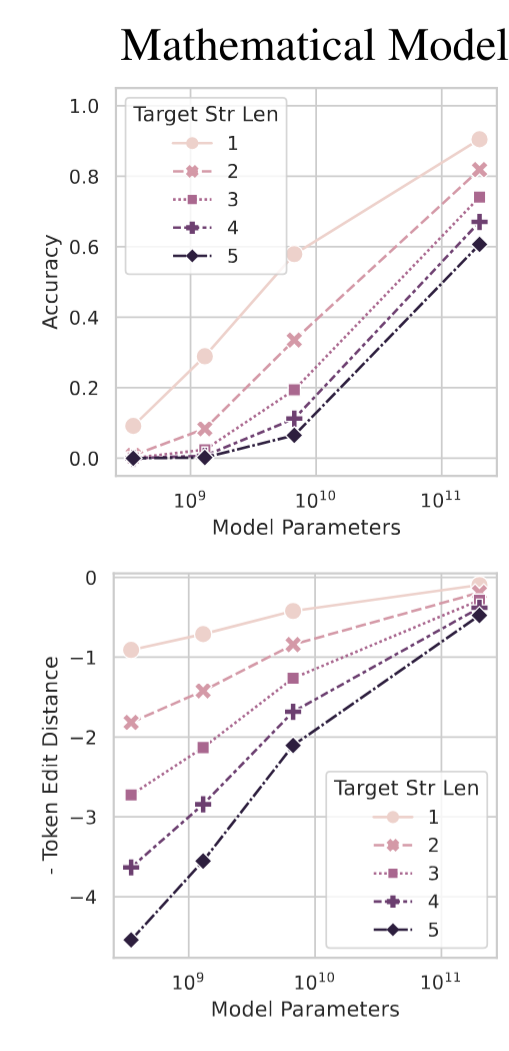
\includegraphics[width=0.3\linewidth]{part1/visuals/token_edit.png}
    \caption{把指标从非线性（上）换成平滑（下）后，所谓涌现能力便消失了 \citep{schaeffer2023emergent} }
    \label{fig:emergent}
\end{figure}




\subsection{逆缩放}
大多数任务随规模提升而改善，但有些任务表现出\emph{逆缩放}：更大的模型表现更差，或发展出更强的偏见。这可能发生在这样的任务中——按语言建模目标，干扰项答案比正确答案概率更高，从而使更大（也更自信）的模型一致地选择错误选项 \citep{mckenzie2023inverse, michaelov-bergen-2023-emergent}。

逆缩放的一个例子是\emph{后见之明忽视}，这项任务检验模型能否根据期望值判断一笔赌注是否值得下。若期望值为正，模型应回答{\em 是}；若期望值为负，则应回答{\em 否}。情形如下：模型只被展示少样本示例，其中实际结果总是与期望值一致（即期望值为正时赌徒赢了钱，期望值为负时输了钱）。然后询问模型：在一笔期望值与实际结果不一致的赌注中，下注是否正确。后见之明忽视检验的是：当少样本示例标注正确但具有误导性时，模型能否从指令中正确泛化。重复代数则检验模型在给定特定模式的、标注正确的少样本示例时，如何回应简单的代数问题。图~\ref{fig:negative-scaling} 表明，模型通常从随机水平起步，但在约 $10^{22}$ 训练 FLOPs 处跌破随机水平。

\begin{figure}
    \centering
    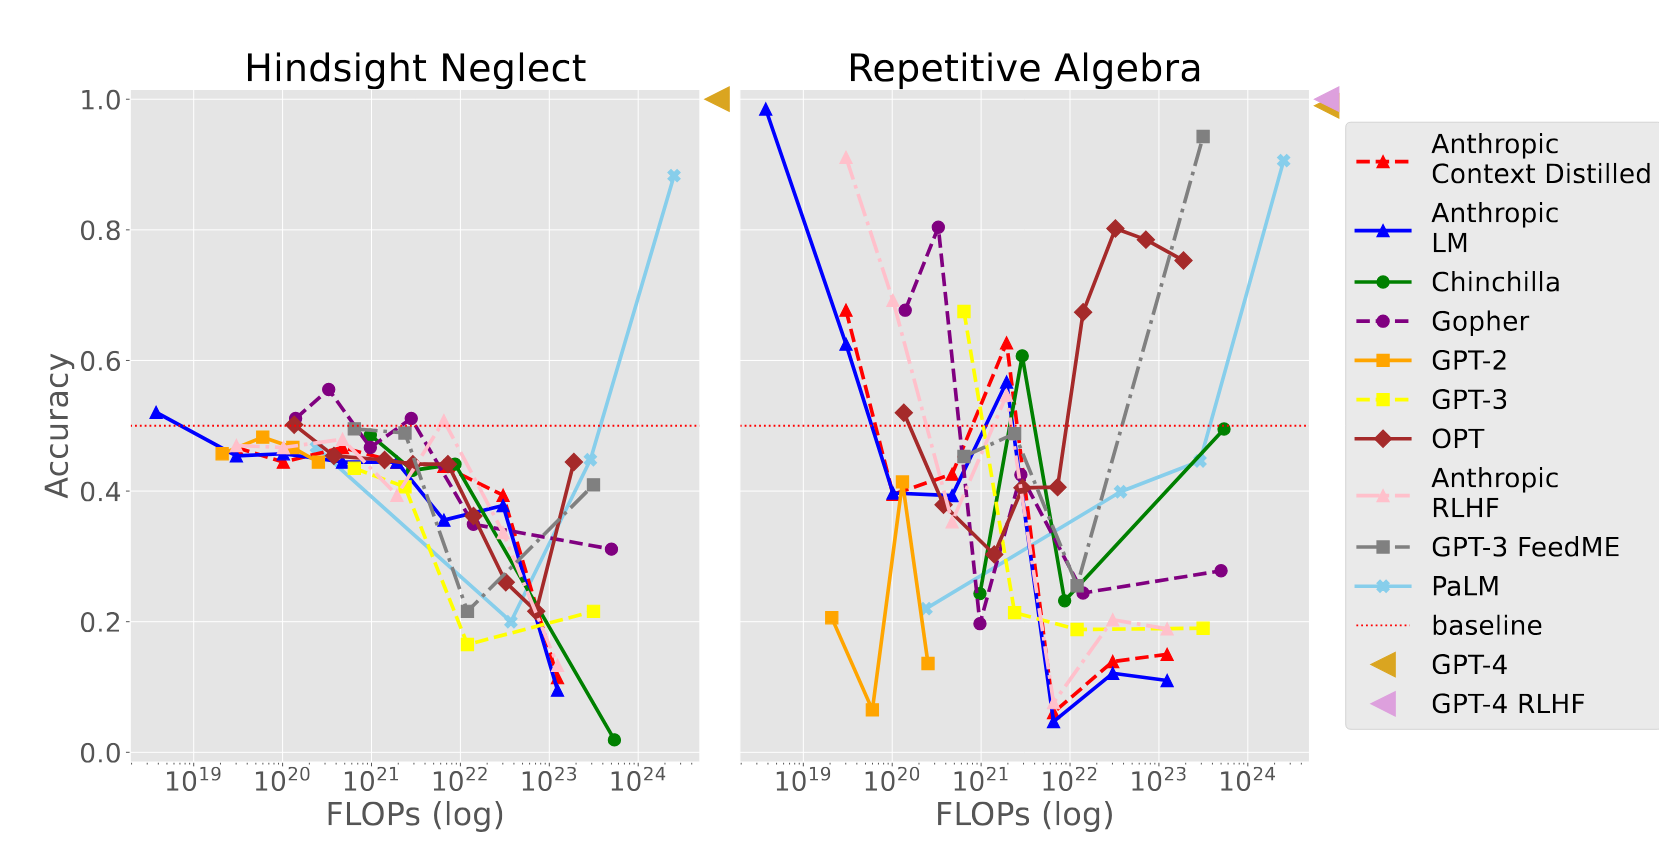
\includegraphics[width=0.8\linewidth]{part1/visuals/negative_scaling.png}
    \caption{后见之明忽视（左）与重复代数（右）任务的缩放行为 \citep{mckenzie2023inverse}}
    \label{fig:negative-scaling}
\end{figure}


\subsection{顿悟（Grokking）}
顿悟是统计学习理论中一个较新的悖论。该理论认为，按常规，当一个大型模型面对一个小数据集时，它会因为记忆示例而过拟合。而顿悟则发生在：我们继续训练这个过大的模型，在更多得多的训练之后，模型突然找到了一个可泛化的解 \citep{power2022grokkinggeneralizationoverfittingsmall}。

虽然最初是在小型算法任务（如模加法）上观察到的，但顿悟现象表明：扩展训练步数（过度训练）可以带来从记忆到理解的质变，即便不增大数据集规模 $D$，见图~\ref{fig:grokking}。

\begin{figure}
    \centering
    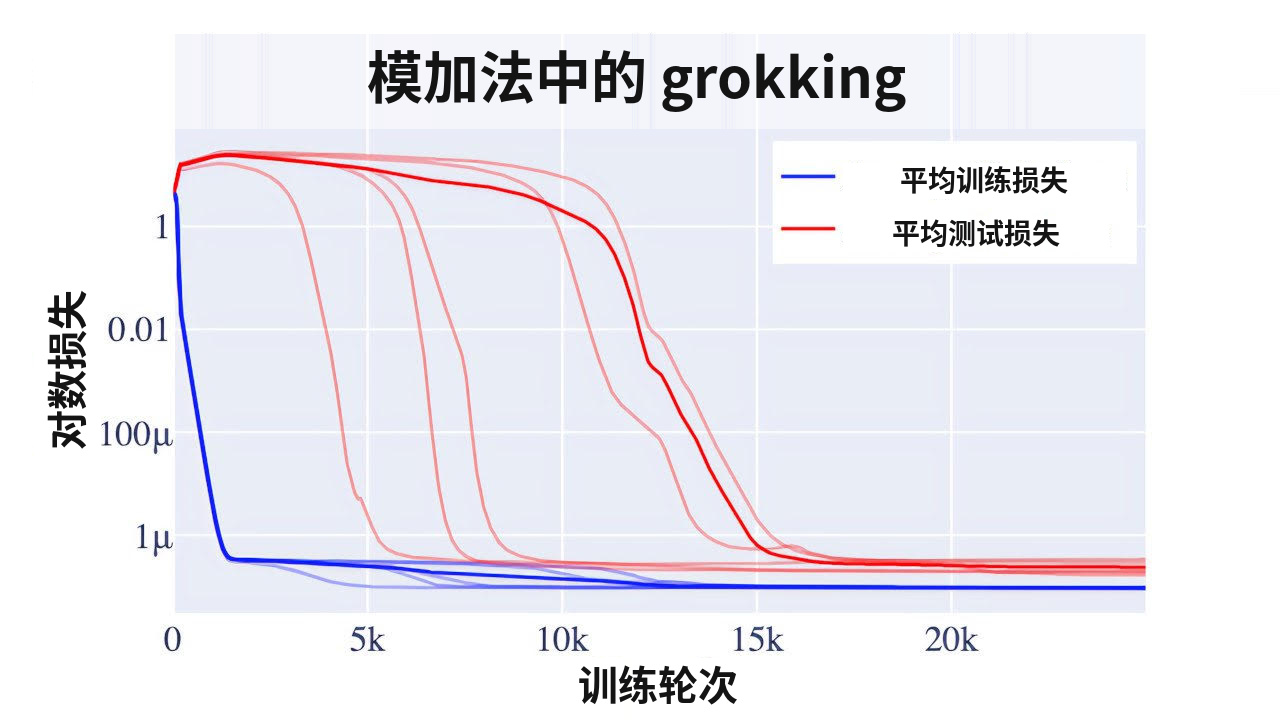
\includegraphics[width=.6\linewidth]{part1/visuals/Grokking_modular_addition.jpg}
    \caption{模加法任务上早期对训练集的记忆（蓝）与后期泛化（红：顿悟）的对比 \citep{nanda2023progress}}
    \label{fig:grokking}
\end{figure}


该图显示了一道「数据墙」：随着数据逐渐耗尽，它起初限制了缩放 \citep{villalobos2024position}；但后来在更多得多的训练之后，模型顿悟出一个可泛化的解。  

顿悟与语言建模相关，因为我们正在迅速耗尽互联网上高质量的人类文本，无法满足下一代模型对 Chinchilla 缩放所要求的 $D$。由于这些固有极限，研究者正把目光投向简单地扩展 $D$ 之外。作为替代，我们可以考察若干这类新前沿：
%\begin{enumerate*}[label=(\arabic*)]
%    \item 
（1）更好的架构效率（例如混合专家）；
%    \item 
（2）推理时缩放（例如在推理时给模型更多算力让它{\em 思考}，如 OpenAI 的 o 系列所示）；或
%    \item 
  （3）合成数据生成（第~\ref{chap:synthetic-data} 章）。
%\end{enumerate*}


\section{小语言模型}
\label{sec:small-models}
随着对算力与数据的要求持续增长，人们对\emph{小语言模型}（SLM）的兴趣日益浓厚：这类模型小到足以在消费级硬件、甚至移动或边缘设备上运行，同时保持高性能。这些模型通常采用在效率上做优化、又不牺牲太多性能的技术来开发。

要理解这类模型的部署格局，把常见的算力基础设施分类会很有帮助：
\begin{itemize}
    \item 数据中心：高性能 GPU（如 NVIDIA H100）与 TPU，主要用于{\em 预训练}大型模型，并承载高吞吐量的推理 API。
    
    \item 消费级硬件：标准台式机 GPU 与高端 CPU，个人用户可以在此以可负担的成本{\em 微调} SLM 或在本地运行它们。
    
    \item 边缘设备：手机、物联网设备与笔记本电脑，它们越来越多地配备专为低功耗、高效设备端{\em 推理}而设计的神经处理单元（NPU）。
\end{itemize}

要把模型装进后两类受限环境，优化技术聚焦于加速吞吐量、降低延迟、减少内存占用并提升样本效率。实现这些目标的技术可分为两类：（1）以模型为中心的优化，针对模型的架构及其优化方式；（2）以数据为中心的优化，针对用于训练模型的数据。我们两类都会讨论。

\subsection{以模型为中心的优化}
我们先讨论以模型为中心的优化技术。
我们介绍以下技术，它们能在保持高任务性能的同时高效训练较小的模型。
以模型为中心的技术可以聚焦于预训练/微调，或聚焦于推理。

\subsubsection{降低预训练成本}

\paragraph{参数高效微调（PEFT）}

诸如{\em 低秩适配}（LoRA）\citep{hu2021lora} 之类的方法，只训练模型参数中极小的一部分（常常 $<1$\%）就能让大模型适配新任务 \citep{lialin2023scaling}。关键观察是：微调中学到的权重更新具有较低的{\em 内在秩}：尽管预训练权重矩阵
$W_0 \in \mathbb{R}^{d \times k}$
是满秩的，把它适配到新任务所需的改变量 $\Delta W$ 却可以用一个低秩矩阵很好地近似。LoRA 不直接更新 $W_0$，而是将其冻结，并把更新表示为两个小矩阵之积，
\begin{equation}
    W = W_0 + \Delta W = W_0 + B A, \qquad B \in \mathbb{R}^{d \times r}, \;\; A \in \mathbb{R}^{r \times k}
\end{equation}
其中秩 $r \ll \min(d, k)$。对输入 $x$，修改后的前向传播变为
\begin{equation}
    h = W_0 x + \frac{\alpha}{r}\, B A x,
\end{equation}
其中 $\alpha$ 是一个常数缩放因子，控制更新的幅度，大致相当于标准训练中的学习率。这一做法见图~\ref{fig:lora}。我们只为 $A$ 与 $B$ 计算权重更新，把可训练参数从 $d \times k$ 减少到 $r(d + k)$。初始化时 $A$ 取自随机高斯分布、$B$ 设为零，因此 $\Delta W = 0$，训练从预训练模型出发。由于 $\Delta W$ 在训练后可以直接合并回 $W_0$，LoRA 不增加推理延迟，而且一个基础模型可以搭配许多小的、可替换的任务专用适配器来提供服务。

\begin{figure}[t]
    \centering
    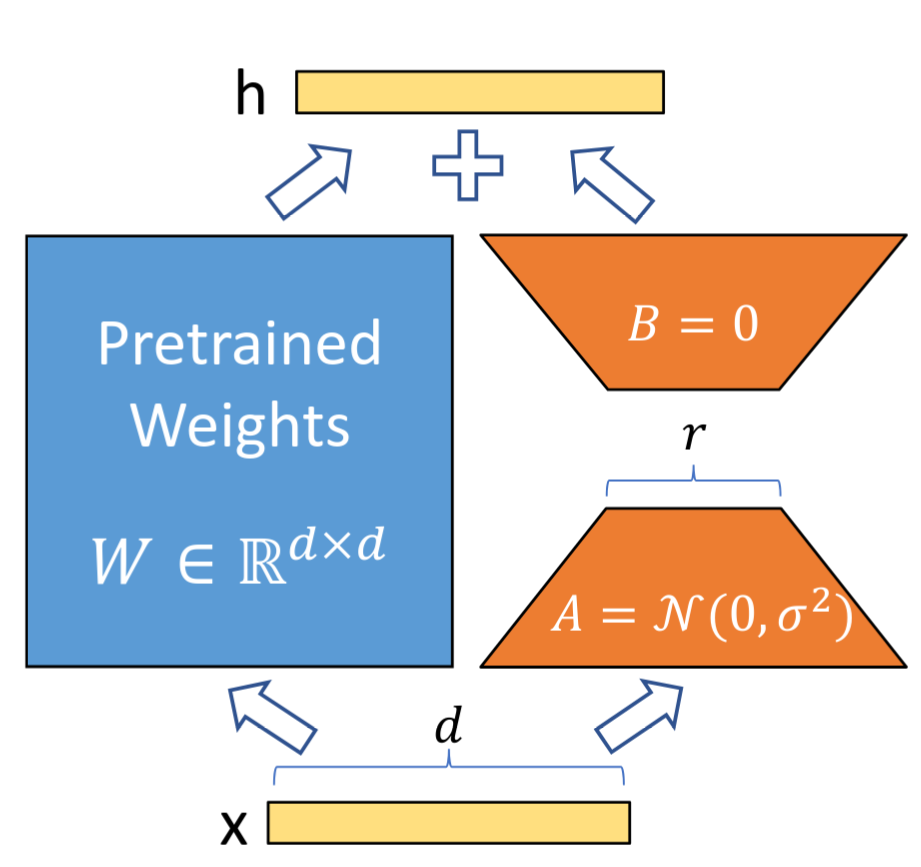
\includegraphics[width=.45\linewidth]{part1/visuals/lora.png}
    \caption{低秩适配的重新参数化 \citep{hu2021lora}。微调期间只训练 $A$ 与 $B$}
    \label{fig:lora}
\end{figure}    

\paragraph{架构创新}
第二类技术直接改变模型架构本身，使其运行更便宜，而不是事后压缩一个固定的架构。两个有影响力的例子是分组查询注意力与混合专家。

\textit{分组查询注意力}（GQA）\citep{ainslie-etal-2023-gqa} 针对的是自回归解码的内存带宽瓶颈。在标准\emph{多头注意力}（MHA）中，每个查询头都有自己的键矩阵与值矩阵，计算注意力分数时都要用到。在另一个极端，\emph{多查询注意力}（MQA）让所有查询头共享单个键/值头，这缩小了计算量，但可能损害表达质量与训练稳定性。GQA 在两者之间插值：把查询头分成 $g$ 组，同组内所有头共享一个键/值头。$g = 1$ 时等价于 MQA，$g$ 等于头数时等价于 MHA，因此 $g$ 在质量与内存占用之间做取舍。GQA 常与下一节第~\ref{sec:small-models} 节讨论的 KV 缓存优化结合使用，如今它已是许多开放权重模型的默认注意力变体。

\textit{混合专家}（MoE）\citep{shazeer2017outrageouslylargeneuralnetworks} 把参数总量与每个词元所花的算力解耦。MoE 层不再在每层放一个稠密前馈块，而是包含许多并行的「专家」子网络，外加一个轻量的\emph{门控网络}（路由器），它为每个词元只激活少量专家（通常是得分最高的 1 或 2 个）。由于只有被选中的专家参与计算，即便参数总量（因而模型的整体容量）增长一个数量级甚至更多，每词元成本仍接近单个稠密块的水平 \citep{JMLR:v23:21-0998}。

这种\emph{稀疏激活}正是 Mixtral 以及许多近期前沿系统能够拥有数千亿总参数、却每个词元只激活其中一小部分的原因。其代价有三：（1）所有专家仍必须常驻内存；（2）负载必须在专家之间均衡（常通过一个辅助损失），以免某些专家被过度使用或闲置；（3）路由引入了额外的工程复杂度。MoE 架构见图~\ref{fig:moe}，图中展示了 top-$k$ 路由机制，配置为 $k=2$，门控函数依据路由器为每个词元选出得分最高的两个 FFN 专家。被选中的专家并行求值，其输出通过加权求和聚合 \citep{zhang2025mixtureexpertslargelanguage}。

\begin{figure}[t]
    \centering
    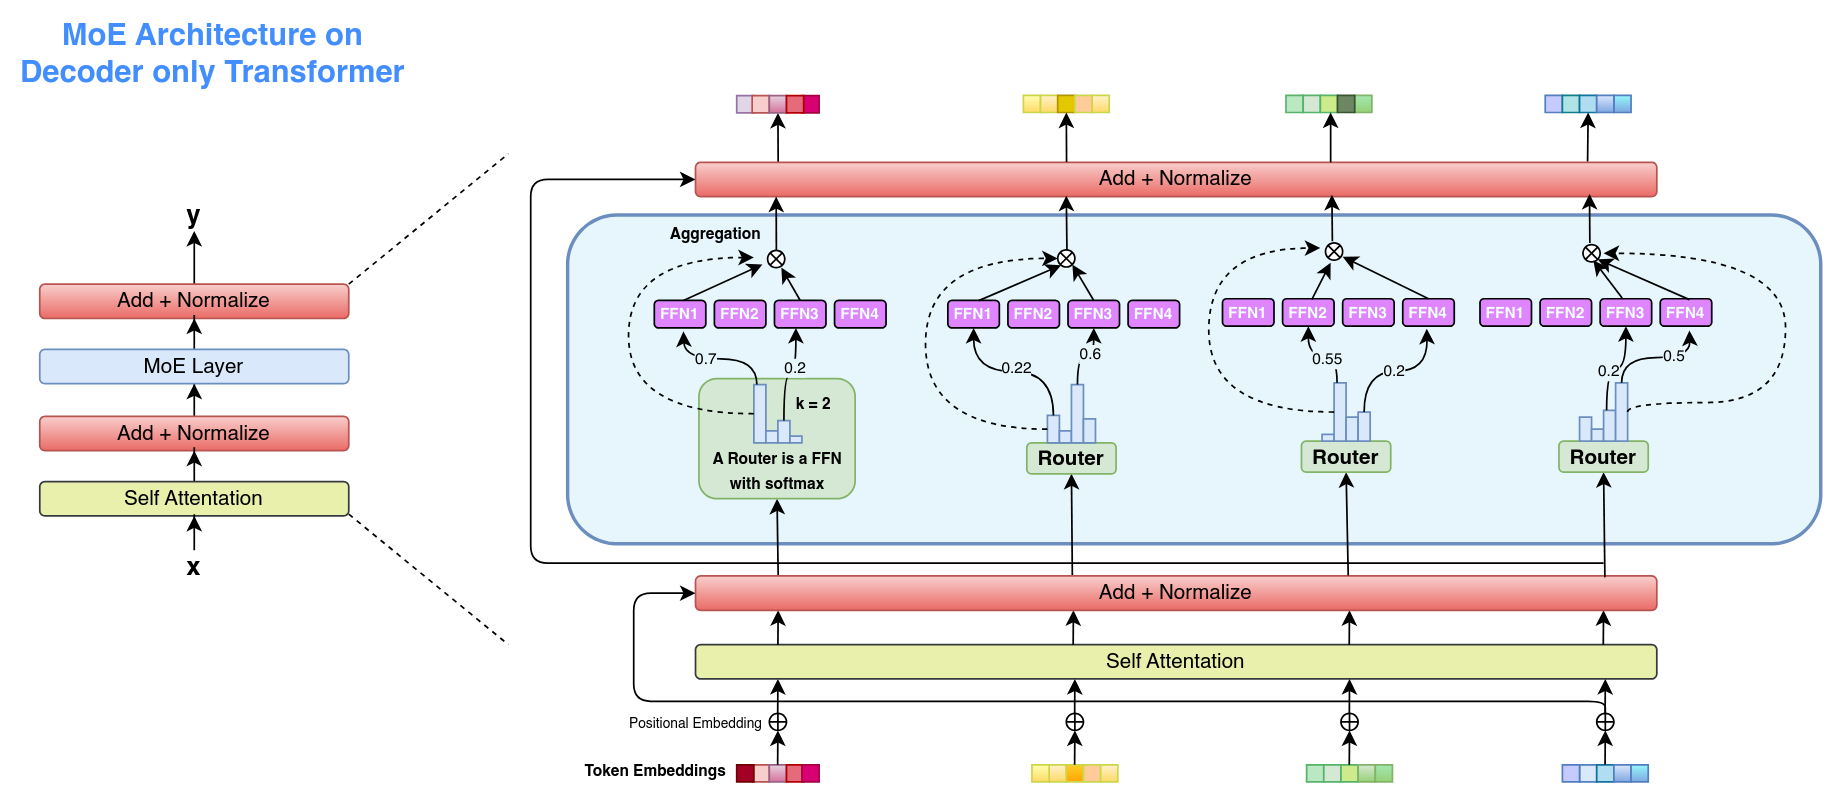
\includegraphics[width=.95\linewidth]{part1/visuals/moe.png}
    \caption{在仅解码器 Transformer 之上稀疏门控的混合专家（MoE）架构示意 \citep{zhang2025mixtureexpertslargelanguage}}
    \label{fig:moe}
\end{figure} 

\paragraph{知识蒸馏}
用一个大的教师模型来训练一个更小的学生模型，办法是促使学生的输出分布与教师匹配 \citep{gu2023minillm, xu2024survey}。关键在于，学生学到的是教师完整的\emph{软}概率（通常用温度来软化），而不只是那一个正确答案。这些软目标携带更丰富的信息：例如教师认为哪些错误答案是可信的。这使学生能以远小于教师的规模接近教师的质量。同一思想也是下文所讨论的合成数据生成的基础——在那里，前沿模型实际上充当教师，为更小的学生模型生成高质量训练数据。


\subsubsection{降低推理成本}
模型训练完成后，还可以针对推理时的部署做进一步优化。训练时技术关注的是降低「产出模型」的成本，而推理时技术针对的是\emph{使用}模型的成本：吞吐量（每秒生成的词元数）、延迟（到首个词元及后续每个词元的时间）以及服务一次请求所需的内存占用。我们讨论几种常用于降低推理成本的技术，它们对大模型和小模型都适用。

\paragraph{键值（KV）缓存} 在自回归生成中，模型一次产生一个词元，而每个新词元都要关注此前所有词元。每一步都为整个上下文重新计算注意力的键与值，代价是平方级的。然而当我们预测一个新词元时，上下文保持不变。我们可以把过去词元的键向量与值向量存入一个\emph{KV 缓存}并复用，而不是重新计算注意力值。这把每步注意力变成了线性代价的查表。这是让解码变得可行的基本优化，但它也有代价：缓存随序列长度与批大小线性增长，在长上下文下很快主导内存占用。这一问题既促成了上述架构选择（GQA 与 MQA 通过让查询头共享键/值头来缩小缓存），也催生了专门的内存管理方案，例如 \emph{PagedAttention}——它把缓存存放在非连续的块中，以减少碎片并提升服务吞吐 \citep{kwon2023efficient}。

\paragraph{剪枝} 一种更极端的缩小模型规模的方法，是考虑移除神经网络中冗余或不重要的连接 \citep{ma2023llm}。剪枝可以是\emph{非结构化}的（把单个权重置零），也可以是\emph{结构化}的（移除整个神经元、注意力头或层）；后者能在标准硬件上带来实际的加速，而前者需要具备稀疏感知能力的算子才能兑现其好处。

\paragraph{量化} 另一种在推理时节省内存的方法，是缩小需要载入内存的矩阵的规模。除了把矩阵维度做小，我们也可以降低权重元素的精度（例如从 16 位降到 8 位或 4 位）。这能显著减少内存占用并加速推理。但原则上，精度越低意味着性能越低。同一思路也可用于 KV 缓存本身，以便把长上下文保持在内存中。量化是一种常用方法 \citep{dettmers2022gpt3, dettmers2023case, xiao2023smoothquant}。

或者，不是把所有权重都转成同一精度，人们提出了\emph{混合精度}模式，对计算的不同部分使用不同的数值精度，以平衡速度与稳定性 \citep{micikevicius2017mixed}。这种做法可能因数值不稳定而出现非确定性结果 \citep{yuan2025understanding}。

\paragraph{推测解码} 优化推理效率的一项关键技术是\emph{推测解码} \citep{leviathan2023fast}。这种做法先用一个小草稿模型快速生成多个词元，再由更大的目标模型并行验证它们。这能在不牺牲大模型质量的前提下加快推理（最高可达 2–3 倍加速），实际上是在利用缩放曲线上不同的点。



\subsection{以数据为中心的优化}
除了以模型为中心的方法，文献还强调：在训练高效模型时，数据质量与数据整理往往比数据集规模更重要 \citep{luo-etal-2025-survey}。小模型若在高度精挑细选的高质量数据上训练，也能表现良好。因此，除了高效的模型架构，构造一份好的数据配方也很重要。以数据为中心的技术大致分为两派：从更广的数据池中\emph{挑选}最有用的部分，以及在优质数据稀缺之处\emph{生成}新的合成数据。

\subsubsection{数据选择与整理}
越来越多的研究表明，与其在全部可用文本上训练，不如仔细挑选\emph{哪些}数据参与训练、以及以何种比例参与，这样在相同算力预算下能得到更好的模型。在预训练方面，NVIDIA 的 \emph{CLIMB} 框架 \citep{diao2026nemotron} 把大规模语料嵌入语义空间、对其聚类，再迭代搜索使代理模型损失最小的数据混合。由此得到的 \emph{ClimbMix} 数据集（4000 亿词元）让一个参数量不足十亿的模型超越了在更大但未过滤语料上训练的同类模型。同一原则也适用于微调阶段：\emph{LIMA} \citep{zhou2023lima} 表明，仅用 $1{,}000$ 对精心挑选的提示词—回答进行监督微调，就足以产出一个强大的指令遵循模型，这支持了这样一种观点：大部分知识是在预训练阶段获得的，而对齐主要是在教模型一种期望的回答\emph{风格}。

\subsubsection{合成数据采集}
当合适的数据并不存在时，可以把它生成出来。{\em 教科书就够了}（Textbooks Are All You Need）这一做法用于微软 Phi 系列等模型 \citep{gunasekar2024textbooks}，它表明在干净、达到教科书质量的合成数据上训练，能让一个仅 13 亿参数的相对较小的模型超越规模为其十倍的模型。

这类流水线通常依靠前沿模型来生成数据，配合{\em 大模型作为评判者}（LLM-as-a-judge）打分来筛选最准确、最具教学价值的样本，并做严格的\emph{去污染}，以确保合成数据不会泄露基准测试集、虚高所报告的性能。这种做法对推理数据尤其有价值：通过在更大模型产出的逐步推理轨迹上训练，可以把复杂的问题求解能力蒸馏进一个更小的架构（另见第~\ref{chap:reasoning} 章）\citep{muennighoff2025s1, arora2026training}。

\subsubsection{样本高效学习}
除合成数据之外，人们越来越关注模型如何从有限的自然数据中更高效地学习。诸如 \emph{BabyLM 挑战赛} \citep{warstadt-etal-2023-findings} 之类的倡议，聚焦于在严格的数据约束下（例如 1000 万到 1 亿词元）训练模型。这与人脑儿童在发育早期接收的语言输入量相当，既推动了样本高效架构的创新，也为认知上合理的语言习得提供了洞见。

\subsection{流行模型}
在综述了各种改进技术之后，看看流行的模型如何把它们付诸实践是有益的。模型通常按开放性分类：闭源权重（专有）模型只暴露 API，开放权重模型发布其训练好的参数，开源模型还额外共享训练数据与代码。在实践中，开放性是一个程度问题而非严格类别，我们之后可能会用一个开放性指数来评定其透明度 \citep{artificialanalysis_openness}。大多数开放模型可以在 Hugging Face 之类的仓库中找到。

下面我们简要介绍一些最流行的开放权重模型，它们被设计得足够高效、可在消费级硬件上运行，以及它们为此采用的技术。这不是一份穷尽的清单，而是在撰写本书时，挑选出的一些有影响力、能体现效率技术趋势及其规模的模型。
\begin{description}[font=\bfseries]
    \item[Phi 系列] \citep{abdin2024phi3technicalreporthighly}。Phi 系列是能力不俗的 SLM，效率高到可以在移动设备上本地运行。Phi 模型背后的核心创新是其以数据为中心的训练方法。微软把经过大量过滤的高质量网页数据与由更大模型生成的合成数据结合起来。这使小模型（如 38 亿参数的 \texttt{Phi-3-mini}）也能表现良好，其推理能力可与 GPT-3.5、Mixtral 等大得多的模型相抗衡。
    \item[Gemma 系列] \citep{gemmateam2024gemmaopenmodelsbased} Google 强调 Gemma 模型继承了 Gemini 强大的通用能力，尤其是在文本、推理与编程方面，同时在其特定规模类别中推进了最先进水平，但外界对其训练方法或数据知之甚少。
    \item[OLMo 家族] \citep{olmo2025olmo3} OLMo（Open Language Model）家族由艾伦人工智能研究所开发，目标是成为完全开源的模型。OLMo 项目开源了完整训练流水线，包括代码与数据：预训练数据集（Dolma）、训练与评估代码、训练日志以及中间检查点。这种透明性使研究者能够研究训练动态、数据影响与算法偏见。
    \item[Qwen 系列] \citep{bai2023qwentechnicalreport} Qwen 家族是一套高性能的基础模型与指令微调模型，从参数量不足十亿的稠密模型一直到大型混合专家（MoE）架构。它们以多语言能力以及在数学、编程和逻辑推理基准上的表现著称。
    \item[OpenELM] \citep{mehta2024openelmefficientlanguagemodel} 苹果的高效语言模型家族，设计目标是在边缘设备上高效运行。其逐层缩放策略让靠近输入的层使用较小的潜在维度、靠近输出的层逐步加宽。这使低参数量下也能获得高准确率。
    \item[gpt-oss] \citep{openai2025gptoss120bgptoss20bmodel} OpenAI 发布的两个开放权重推理模型，采用高效的混合专家架构，针对智能体能力做了优化。
    \item[Mixtral 系列] \citep{jiang2024mixtralexperts} 这些模型把稀疏混合专家（SMoE）架构带入了开放权重生态（如 Mixtral 8x7B），使模型可以拥有很大参数量、而推理时只激活少量参数，从而最大化效率。
    \item[Llama 系列] \citep{grattafiori2024llama3herdmodels} Meta 的 Llama 模型已被广泛使用。它们在大规模数据集上训练（Llama 3 最多达 15 万亿词元），规模从小巧的、适合边缘设备的尺寸一直到 405B 参数的前沿模型，为开放模型中的缩放定律树立了标杆，并催生了一个由微调模型与衍生物构成的生态。
    \item[DeepSeek] \citep{deepseekai2025deepseekv3technicalreport} DeepSeek-V3 是一个大型混合专家模型（总参数 671B，每词元激活 37B），以其训练的稳定性著称。它把用于压缩键值缓存的多头潜在注意力（MLA）与无需辅助损失的专家负载均衡策略结合起来，并以 FP8 混合精度训练，以较小的算力代价达到了前沿水平的表现。该系列还包括 DeepSeek-R1 推理模型。
    \item[GLM] \citep{glm5team2026glm5vibecodingagentic} 由智谱 AI 开发的 GLM（General Language Model）家族建立在强大的推理能力之上，这些能力在训练早期形成、并在整个训练过程中得以保持。近期版本针对智能体工作流与软件工程做了优化，目标不只是文本补全，还包括工具使用与代码生成性能。
    \item[Pythia] \citep{biderman2023pythia} EleutherAI 的 Pythia 是一套模型（从 70M 到 12B 参数），用于支持对训练动态与缩放的研究。每个模型都用相同的数据、按相同的顺序训练，并为每个模型发布中间检查点，从而能够受控地研究能力、记忆与偏见在训练过程中如何涌现。
    \item[BLOOM] \citep{workshop2023bloom176bparameteropenaccessmultilingual} BLOOM 是 BigScience 协作研究项目产出的 176B 参数开放获取模型。它在覆盖 46 种自然语言与 13 种编程语言的 ROOTS 语料上训练，是最早优先考虑多语言覆盖与完全开放性的大规模模型之一，并按负责任 AI 许可发布。
    \item[SmolLM] \citep{allal2025smollm} Hugging Face 的 SmolLM 是一个紧凑模型家族（135M、360M 与 1.7B 参数），面向高效的设备端部署，与 Phi 系列颇为相似。其性能源于数据整理：它在 SmolLM-Corpus 上训练，该语料融合了高质量网页数据、Python 代码示例，以及由 Mixtral 合成生成的教科书与故事。
\end{description}


% \subsection{Dual System Theory in AI}
% \label{sec:dual-system}
% This shift can be contextualized through the lens of dual system theory \citep{evans2013dual, kahneman2013thinking}, which holds that human cognition consists of two distinct systems. System 1 (``thinking fast'') is automatic, intuitive, and relies on heuristics to efficiently handle everyday tasks without deep analytical precision. Conversely, System 2 (``thinking slow'') is deliberate, logical, and is used to solve complex, novel challenges. Humans utilize metacognition---they monitor their own thought processes---to recognize when to switch from the quick instincts of System 1 to the careful reasoning of System 2.

% Historically, in AI, knowledge- or logic-based systems have been categorized as System 2, whereas modern machine learning methods have been predominantly viewed as System 1 \citep{fabiano2025thinking}. However, the introduction of test-time scaling marks a transition in deep learning toward System 2 capabilities.

% With the advent of large language models (LLMs), a debate has emerged  whether these models can genuinely reason and solve problems autonomously, or if they require distinct symbolic solvers and separate metacognitive agents. The discussion largely revolves around emergent behaviors---such as the ability to solve planning problems or adapt to novel tasks---which the systems were not explicitly trained to handle.

% There are two primary schools of thought on this issue. One position argues that LLMs are merely executing complex next-word prediction based on surface-level statistics, fundamentally lacking the capacity for deliberate, grounded reasoning \citep{bender2021dangers}. Conversely, others point to emergent capabilities as evidence that LLMs can function as both solution generators and models of the world, capable of reasoning over past choices and utilizing memory to plan \citep{hao-etal-2023-reasoning}.
% %
% To navigate this questions, researchers have developed various inference techniques that can be classified as either fast and intuitive (System 1) or deliberative and decoupled (System 2). We will highlight a few examples of these in the following sections.


\section{推理时算力}
\label{sec:inference-time}
% The traditional scaling laws focus on the relationship between compute and performance \textit{at training time}. However, a new frontier has emerged: \emph{inference-time scaling} (or test-time compute) \citep{muennighoff2025s1}. Just as scaling parameters and training data improve a model's capabilities, allocating more compute during inference allows a model to spend more time deliberating to produce a high-quality answer. While the scaling laws discussed so far already account for compute, this compute is solely spent during training. However, in the new paradigm, we add a new computational burden, not in training but in inference. With this shift to test-time compute, we can also start a relevant discussion on what type of systems LLMs are. We will introduce the relevant techniques and concepts in detail in the rest of the book, starting in Chapter~\ref{chap:reasoning}.

% \paragraph{Test-Time Compute and Scaling Laws}
% In addition to the traditional scaling parameters (model size, dataset size, and training compute), test-time scaling introduces an additional variable: the amount of compute utilized at inference time, often measured by the number of tokens generated or paths explored.

% Increasing this parameter can lead to significant improvements in LLM capabilities \citep{du2024improving}. For instance, recent research indicates that optimally scaling test-time compute can allow smaller models to outperform much larger models on difficult reasoning tasks \citep{snell2024scaling}. However, these improvements are not uniformly guaranteed and depend heavily on the nature of the task and the specific search or verification strategies employed \citep{stechly2023gpt}.

传统的缩放定律关注算力与性能在\textit{训练时}的关系。较新的研究把这部分算力负担转移到了推理阶段：\emph{推理时缩放}（或测试时算力）\citep{muennighoff2025s1}。模型不再把所有算力花在训练上，而是在推理时被允许更长时间地斟酌，以产出更高质量的回答。这以生成的词元数或探索的推理路径数来衡量。因此，优化吞吐量（词元/秒）变得至关重要：词元产出越快，模型在同样时间内能做的推理就越多。 

按词元数增加这一推理时预算，可以显著提升能力 \citep{du2024debate}；近期工作表明，最优地分配测试时算力，能让较小的模型在困难推理任务上超越更大的模型 \citep{snell2024scaling}。不过这些收益并非必然，它取决于任务以及所采用的特定搜索或验证策略 \citep{stechly2023gpt}。除性能之外，这一转变也重新提出了一个更宽泛的问题：LLM 究竟属于哪一类系统——我们将在第~\ref{chap:reasoning} 章详细讨论。


\section{可持续语言模型}
\label{sec:sustainable}
LLM 训练与部署的巨大规模带来了显著的环境与经济影响。AI 训练与推理的能耗很大，%the amount of hardware and infrastructure required may scale beyond the amount of compute available in the world so far, 
随之而来的冷却用水也给供水管网带来压力 \citep{10.1145/3724499, jegham2025hungryaibenchmarkingenergy}。衡量训练的能源使用与碳足迹，直到最近才进入标准报告范畴 \citep{ding2024sustainable}。据报道，训练单个大模型的能耗可相当于数百个家庭一年的用电量。训练像 BLOOM 这样的模型，在同时计入动态功耗与硬件制造中的隐含碳排放后，排放了超过 50 吨二氧化碳当量 \citep{JMLR:v24:23-0069}。

随着 LLM 在科学与社会的使用日益增加，总碳足迹越来越由\emph{推理}而非训练主导，对于每天被数百万人使用的模型尤其如此 \citep{ozcan2025quantifying, wu2022sustainable, samsi2023words}。这带来一个机会：在训练时投入更多算力以造出更小、更高效的模型（如第~\ref{sec:scaling-laws} 节所讨论），可以显著降低部署的长期环境成本。

当全球推理需求扩展到每天数十亿次查询时，累计能耗及相关财务成本会超过最初的训练投入 \citep{faiz2024llmcarbon}。在这一规模上部署大模型需要庞大的数据中心基础设施，以及大量电力与水消耗。因此，人们强烈倾向于部署小语言模型（SLM）以实现可持续的大规模使用。通过把参数量与量化位数降到最低，SLM 降低了每生成一个词元所需的内存带宽与算力，提供了一种更绿色、经济上更可行的方案。

\paragraph{隐私与数据泄露}
除环境问题之外，通过云 API 集中使用 LLM 也带来了隐私漏洞。当用户查询云端模型时，敏感的个人数据、企业知识产权或受保护的健康信息都必须传输到第三方服务器。这会造成数据泄露风险 \citep{aiyappa-etal-2023-trust, li2024opensourcedatacontamination}，途径可能是未授权的拦截、对抗性提取攻击，或模型无意中记住了用户的私密提示词并随后原样吐出 \citep{chen2024janus, maini2024llm, liu2022membership}。

为缓解这些隐私风险并减少对云基础设施的依赖，开发者可以从基于 API 的推理转向\emph{本地、设备端推理} \citep{qu2025mobile}：
\begin{itemize}
    \item 基于 API 的推理：依赖强大的远程服务器。这虽然能访问拥有数千亿参数的前沿模型，但受制于网络延迟、需要持续联网，并且天然会把用户数据暴露给云服务商。
    \item 本地推理：直接在用户硬件（如智能手机、笔记本电脑或边缘服务器）上运行模型。这既保证了数据隐私——提示词从不离开设备，又消除了网络延迟、保证离线可用。
\end{itemize}
%
本地推理受消费级与边缘硬件的物理极限约束。例如内存与带宽有限。LLM 推理是一个受内存约束的过程：存储模型权重需要可观的 RAM 容量，而生成词元则需要高内存带宽。此外，大多数移动设备靠电池供电。在移动设备或标准笔记本上运行密集的矩阵乘法，会导致电池快速耗尽与热降频。

要让本地部署可行，开发者必须依靠推理时优化技术，例如量化（如 4 位）与推测解码，同时也要依靠越来越多专为低功耗边缘 AI 设计的专用神经处理单元（NPU）。


\section{结语}
随着 LLM 的使用日益普及、对快速响应的需求不断增加，LLM 开发的重心正转向更高效的方案。因此，纯粹为追求原始性能而扩展数据、算力与模型规模的重心，正在转变为为\emph{效率}而缩放的重心。 

虽然基本的幂律依然成立，但重心已从「训练尽可能大的模型」转向算力最优训练、推理时缩放，以及开发能在消费级与边缘硬件上运行的高能力小模型。 

本章讨论的这些方向是互补而非竞争的：以模型为中心的技术（LoRA、GQA、MoE、量化、蒸馏）与以数据为中心的技术（细致的数据选择与合成生成）正越来越多地在同一份训练配方中结合使用。 

随着我们越来越逼近数据墙，合成数据与架构效率的作用可能会愈发重要，「以更少做更多」的能力正成为研究焦点。


\bibliographystyle{plainnat}
\bibliography{agenticbook,refs,case,synthetic}
